\documentclass{article}
\usepackage{graphicx}
\usepackage{listings}
\usepackage{ctex}
\usepackage{graphicx}
\usepackage[a4paper, body={18cm,22cm}]{geometry}
\usepackage{amsmath,amssymb,amstext,wasysym,enumerate,graphicx}
\usepackage{float,abstract,booktabs,indentfirst,amsmath}
\usepackage{array}
\usepackage{booktabs} %调整表格线与上下内容的间隔
\usepackage{multirow}
\usepackage{diagbox}
\usepackage{indentfirst}
\usepackage{bm}
\usepackage{fancyhdr}




\pagestyle{fancy}

\lhead{\bfseries \normalsize 学号:1952033\quad 姓名:侯雅玥 \quad 组员:廖宏 \\实验名称:集成移位寄存器应用实验\quad 课程名称:电子技术实验\quad 专业:微电子科学与工程 } 
\rhead{}

\begin{document}
	\section{\zihao{4} 实验名称:集成移位寄存器应用实验}
    \section{\zihao{4} 实验目的}
    \zihao {5} (1)熟悉 555 定时器电路结构、工作原理及特点。\par 
               (2)掌握 555 定时器的基本应用。\par
               (3)熟悉用示波器测量 555 定时器的脉冲幅度、周期和脉冲宽度。 \par
   	\section{\zihao{4} 实验原理}
      
       55定时器是由模拟和数字电路相混合构成的集成电路。由于电路中使用了三个 5kΩ的电阻,故取名为 555电路。
       555电路只要外接少量阻容元器件,就可以组成单稳态触发器、多谐振荡器、多种波形发生器等。
       由于电路结构简单,性能可靠,使用方便,故应用范围很广泛。555电路的内部结构框和引脚排列图如图1、图2所示。
       \begin{figure}[h]
        \begin{minipage}[t]{0.5\linewidth} % 如果一行放2个图,用0.5,如果3个图,用0.33  
          \centering   
          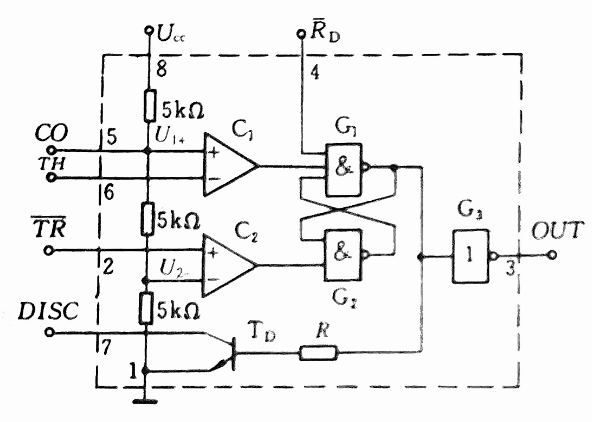
\includegraphics[width=3.5in]{H:/电子技术试验/4-23/4-23-1.png}   
          \caption{555定时器内部结构图}   
          \label{fig:side:a}   
        \end{minipage}%   
        \begin{minipage}[t]{0.5\linewidth}   
          \centering   
          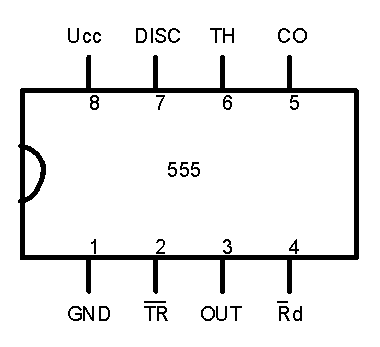
\includegraphics[width=2.5in]{H:/电子技术试验/4-23/4-23-2.png}   
          \caption{555定时器引脚图}   
          \label{fig:side:b}   
        \end{minipage}   
      \end{figure}

      555 定时器主要由两个电压比较器($C_1$和$C_2$)、一个基本 RS触发器、一个泄放三极管 $T_D$和三个5kΩ电阻构成的分压器组成。
      与非门$G_1$和$G_2$,构成基本 RS 触发器,输入$R_D$'为复位端,低电平有效。比较器$C_1$和 $C_2$的输出$U_{C1}$和$U_{C2}$为
       RS触发器的触发信号。若比较器 $C_1(C_2)$的"+"输入端电位低于"一"输入端电位,即 $U_+<U_-$则输出U+为低电平(Uc="0"),
       反之输出Uc为高电平(Uc="1")。比较器C1的参考电压$U_{1+} =\frac{2}{3} U_{CC}$,
      比较器 C2的参考电压 $U_{2_-}=\frac{1}{3}U_{CC}$,如果$U_{1+}$的
      外接端CO接固定电压$U_{CO}$,则$U_{1+} =U_{CO}$,$U_{2_-}=\frac{1}{2}U_{CO}$泄放三极管$T_D$为外接电容提供充、放电回路。
      反相器$G_3$为输出缓冲反相器,起整形和提高带负载能力的作用。\par
      从图2的555定时器引脚排列图可以看出,引脚4为复位端$R_D$'引脚5为电压控制端CO,可以改变比较器$C_1$和$C_2$的上、
      下参考电位$U_{1+}$和$U_{2-}$引脚2为低电平触发端TR;引脚6为高电平触发端 TH;引脚7为$T_D$的集电极开路输出(放电)端DISC。\par
(1)555 定时器构成单稳电路\par
图3为 555 定时器构成的单稳态触发器电路,复位端 $R_D$'接高电平 $U_{CC}$。触发信号ui从低电平触发端TR'输入,所以电路在ui的下降沿触发。
三极管 $T_D$的集电极输出 DISC端通过电阻R 接$U_{CC}$,构成反相器。反相器的输出(DISC)同时接电容 C,555定时器的高电平触发端 TH也与DISC 端相连,
从而构成积分型单稳态触发器。其工作波形如图4所示。\par

\begin{figure}[h]
    \begin{minipage}[t]{0.5\linewidth} % 如果一行放2个图,用0.5,如果3个图,用0.33  
      \centering   
      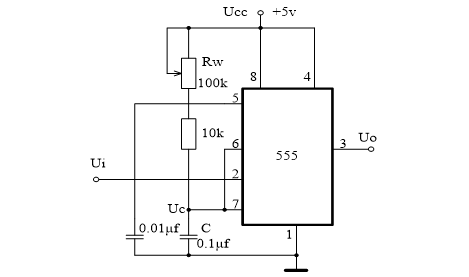
\includegraphics[width=4in]{H:/电子技术试验/4-23/3.png}   
      \caption{555定时器内部结构图}   
      \label{fig:side:a}   
    \end{minipage}%   
    \begin{minipage}[t]{0.5\linewidth}   
      \centering   
      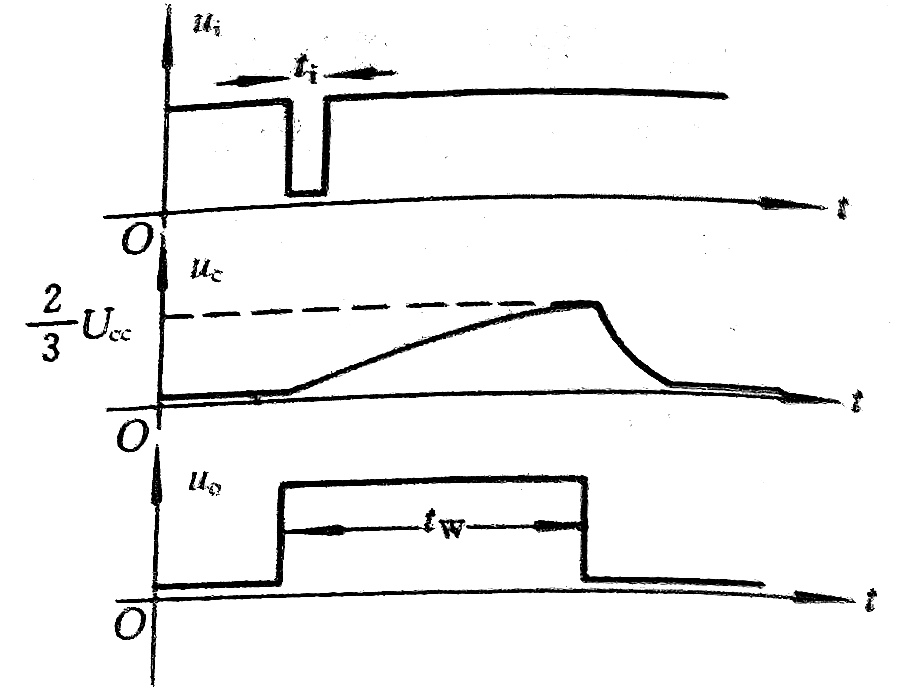
\includegraphics[width=3in]{H:/电子技术试验/4-23/2.jpg}   
      \caption{555定时器引脚图}   
      \label{fig:side:b}   
    \end{minipage}   
  \end{figure}


当 CO端不外接控制电压时,该单稳态触发器的输出脉冲宽度$ t_w$为
\[   t_w=RCln\frac{U_{CC}}{U_{CC}-\frac{2}{3}U_{CC}}\approx 1.1RC  \]
\par
$t_w$由定时元件R与C参数决定,改变 R 与C 值,可以控制输出波形的宽度。因此,单稳态触发器常用于定时、延迟或整形电路。\par
(2)用 555 定时器构成多谐振荡器\par
图5是 555定时器构成多振荡器电路,高、低电平触发输入 TH与TR'相连作为输入。电压控制端CO接0.01μF 电容滤波,$R_D$端接高电平。
三极管$ T_D$集电极上拉电阻 $R_A$至电源$U_{CC}$构成反相器,反相器输出DISC通过$R_BC$积分电路反馈至输人 TH和TR',组成自激多谐热荡器。
此电路没有稳态,也不需外加触发信号,电源通过$R_A$和 $R_B$向C充电以及C通过$R_B$间DISC端放电,使电路自动在两个暂稳态之间变化,
形成振荡信号输出、可以分析,在容充电时,电路的暂稳态持续时间为
\[ t_{w1}=0.7(R_A+R_B)C\]
在电容 C放电时,暂稳态持续时间为
\[t_{w2}=0.7R_BC\]
因此,电路输出矩形脉冲信号的周期为
\[T=t_{w1}+t_{w2}=0.7(R_A+2R_B)C\]
输出矩形脉冲的占空比为
\[q=\frac{t_{w1}}{T}=\frac{R_A+R_B}{R_A+2R_B}\]

可见,通过改变电阻 $R_A$与 $R_B$和电容 C的参数,即可改变振荡信号频率。振荡信号的占空比由$R_A$与 $R_B$的参数决定,但无法小于 
50\%。要使多谐振荡器的占空比在 50\%以下的范围可调,必须使电容的充、放回路互相独立。
那么可以在图5所示电路上增加 1个电位器和2 个二极管来实现,如图 6所示。

\begin{figure}[h]
    \begin{minipage}[t]{0.5\linewidth} % 如果一行放2个图,用0.5,如果3个图,用0.33  
      \centering   
      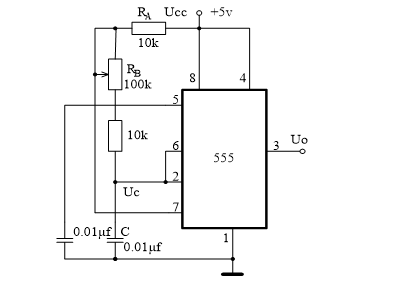
\includegraphics[width=3.5in]{H:/电子技术试验/4-23/4.png}   
      \caption{555定时器内部结构图}   
      \label{fig:side:a}   
    \end{minipage}%   
    \begin{minipage}[t]{0.5\linewidth}   
      \centering   
      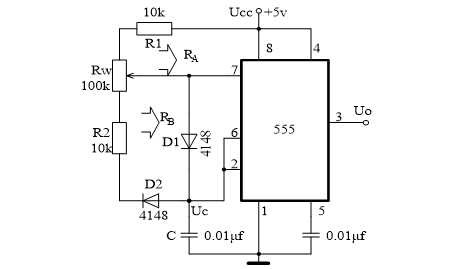
\includegraphics[width=4in]{H:/电子技术试验/4-23/6.png}   
      \caption{555定时器引脚图}   
      \label{fig:side:b}   
    \end{minipage}   
  \end{figure}


\section{\zihao{4} 实验内容及步骤}
1.构成单稳态触发器:按图3接线,C=0.1µF,输入端加1kHz的脉冲信号,用示波器观察Ui,Uc,Uo的波形。改变电位器Rw的阻值,测量输出脉冲宽度tw的变化范围,并与理论值相比较。\par
2.构成多谐振荡器:按图5连接电路,其中,RA为10kΩ电阻,RB由100kΩ电位器和10kΩ电阻串联构成,电容C为0.01µF。调节RB使输出Uo的频率f=1kHz,记录此时的Uo,Uc的波形和RB的实际阻值。\par
3.占空比可调的脉冲信号发生器:按图6连接电路,其中R1=R2=10kΩ,Rw=100kΩ。改变电位器Rw值,组成一个占空比为50\%的脉冲信号发生器,用示波器记录Uo,Uc的波形。Rw变化时,记录占空比的变化范围。(C=0.01µF)\par


\section{\zihao{4} 实验设备和器材}
(1)直流稳压电源              \qquad \quad \qquad \qquad \qquad \qquad           1台\par
(2)数字逻辑实验箱            \qquad  \qquad \qquad \qquad\qquad                1台\par
(3)555             \qquad   \qquad     \qquad \qquad \qquad \qquad \qquad \qquad     1片\par
(4)示波器                   \qquad  \qquad \qquad \qquad\qquad  \qquad  \qquad    1台\par
(5)导线   
\section{\zihao{4} 数据处理}
(1)555单稳态触发器\par
$u_i,u_c$波形
\begin{figure}[h]
    \begin{minipage}[t]{0.5\linewidth} % 如果一行放2个图,用0.5,如果3个图,用0.33  
      \centering   
      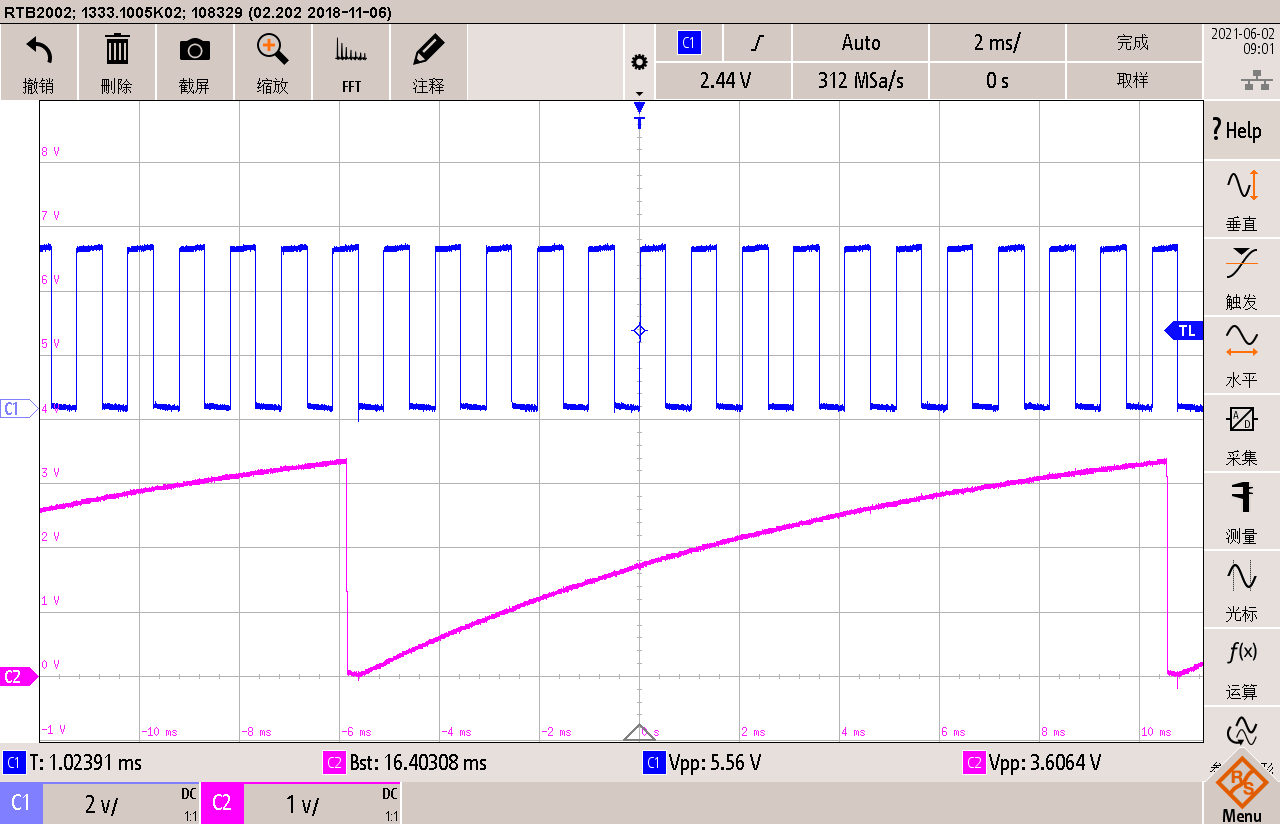
\includegraphics[width=3.5in]{H:/电子技术试验/4-23/SCR28.png}   
      \caption{$R_w=116.2k\Omega$}   
      \label{fig:side:a}   
    \end{minipage}%   
    \begin{minipage}[t]{0.5\linewidth}   
      \centering   
      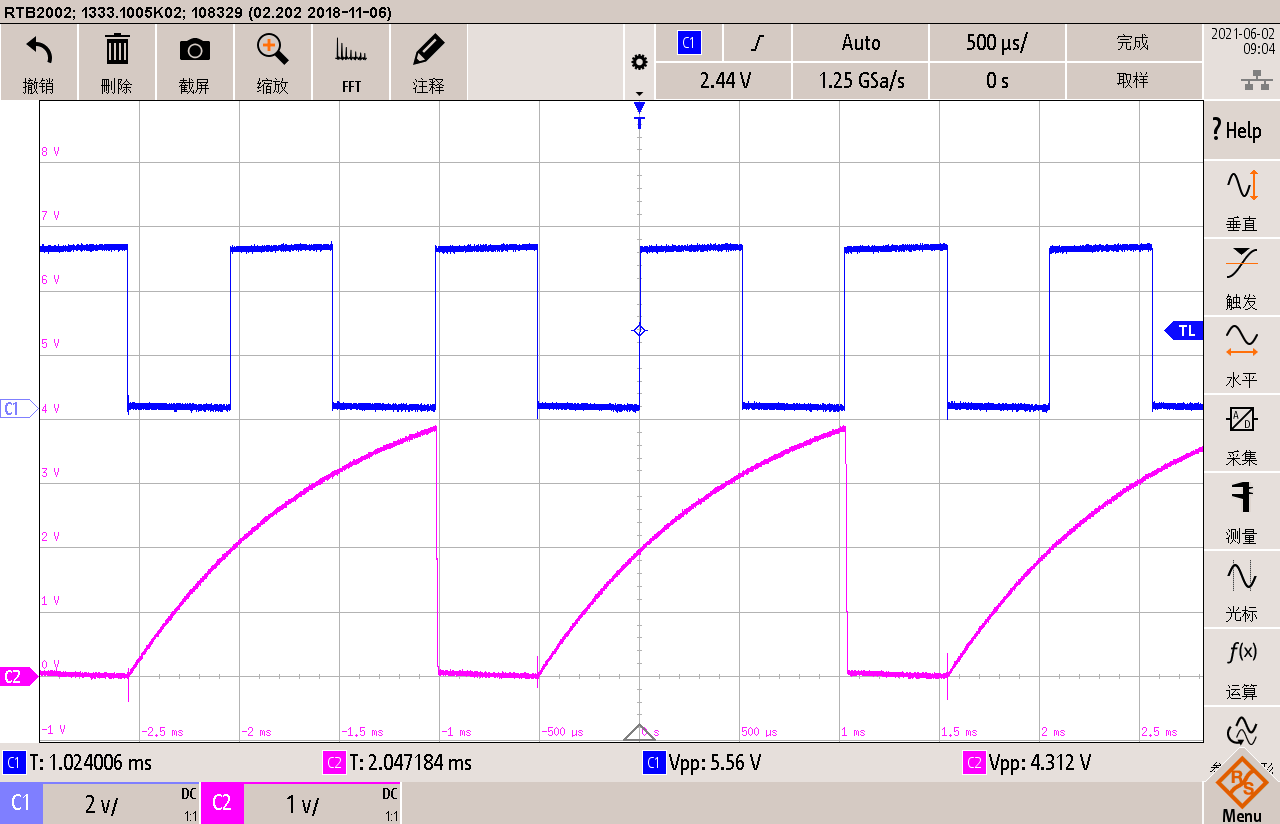
\includegraphics[width=3.5in]{H:/电子技术试验/4-23/SCR31.png}   
      \caption{$R_w=0k\Omega$}   
      \label{fig:side:b}   
    \end{minipage}   
  \end{figure}
  $u_i,u_0$波形
  \begin{figure}[h]
    \begin{minipage}[t]{0.5\linewidth} % 如果一行放2个图,用0.5,如果3个图,用0.33  
      \centering   
      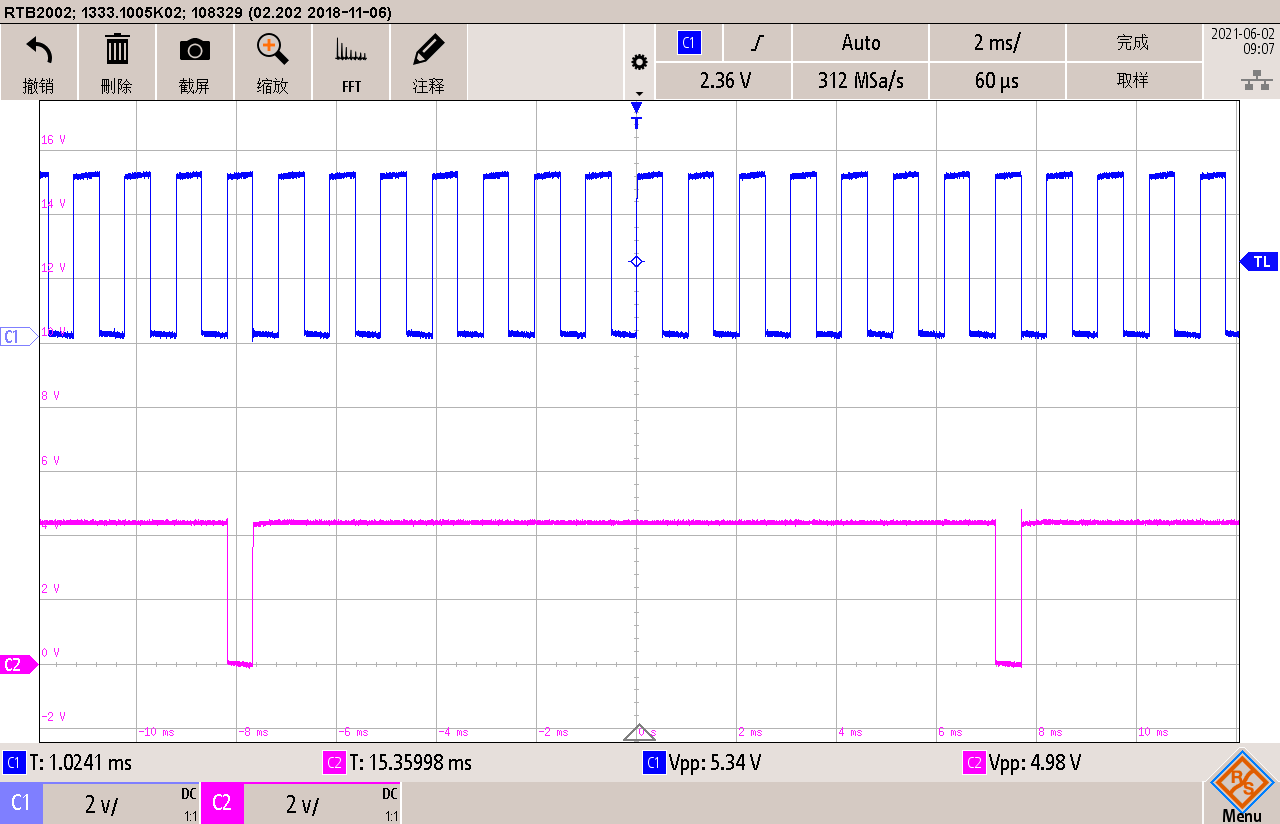
\includegraphics[width=3.5in]{H:/电子技术试验/4-23/SCR34.png}   
      \caption{$R_w=116.2k\Omega$}   
      \label{fig:side:a}   
    \end{minipage}%   
    \begin{minipage}[t]{0.5\linewidth}   
      \centering   
      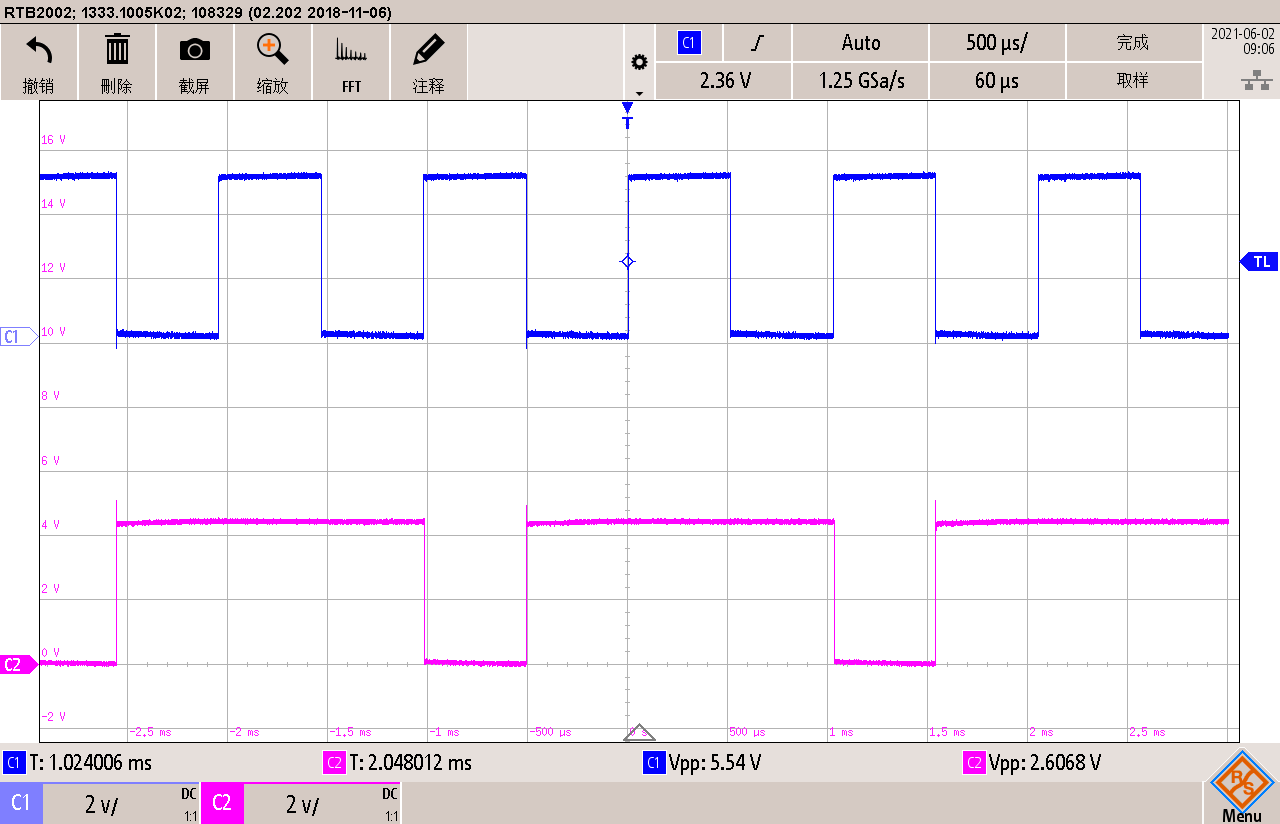
\includegraphics[width=3.5in]{H:/电子技术试验/4-23/SCR33.png}   
      \caption{$R_w=0k\Omega$}   
      \label{fig:side:b}   
    \end{minipage}   
  \end{figure}

\newpage
  (2)多谐振荡器\par
  $u_i,u_c$波形
  \begin{figure}[h]
        \centering   
        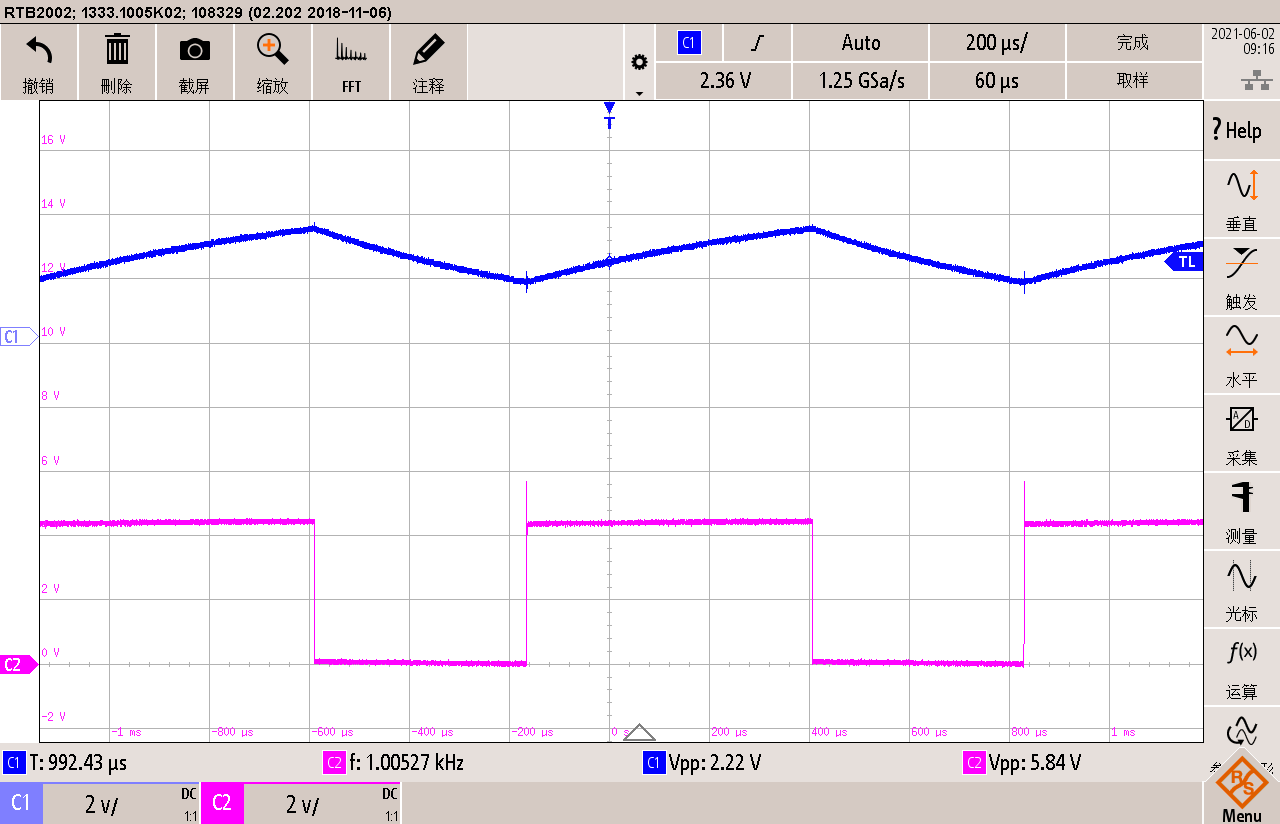
\includegraphics[width=3.5in]{H:/电子技术试验/4-23/SCR35.png}   
        \caption{$U_0,U_c$}   
        \label{fig:side:a}   
    \end{figure}
\par
此时测得$R_B=41.3k\Omega$
\par
(3)占空比可调的脉冲信号发生器\par
  $u_0,u_c$波形
  \begin{figure}[h]
        \centering   
        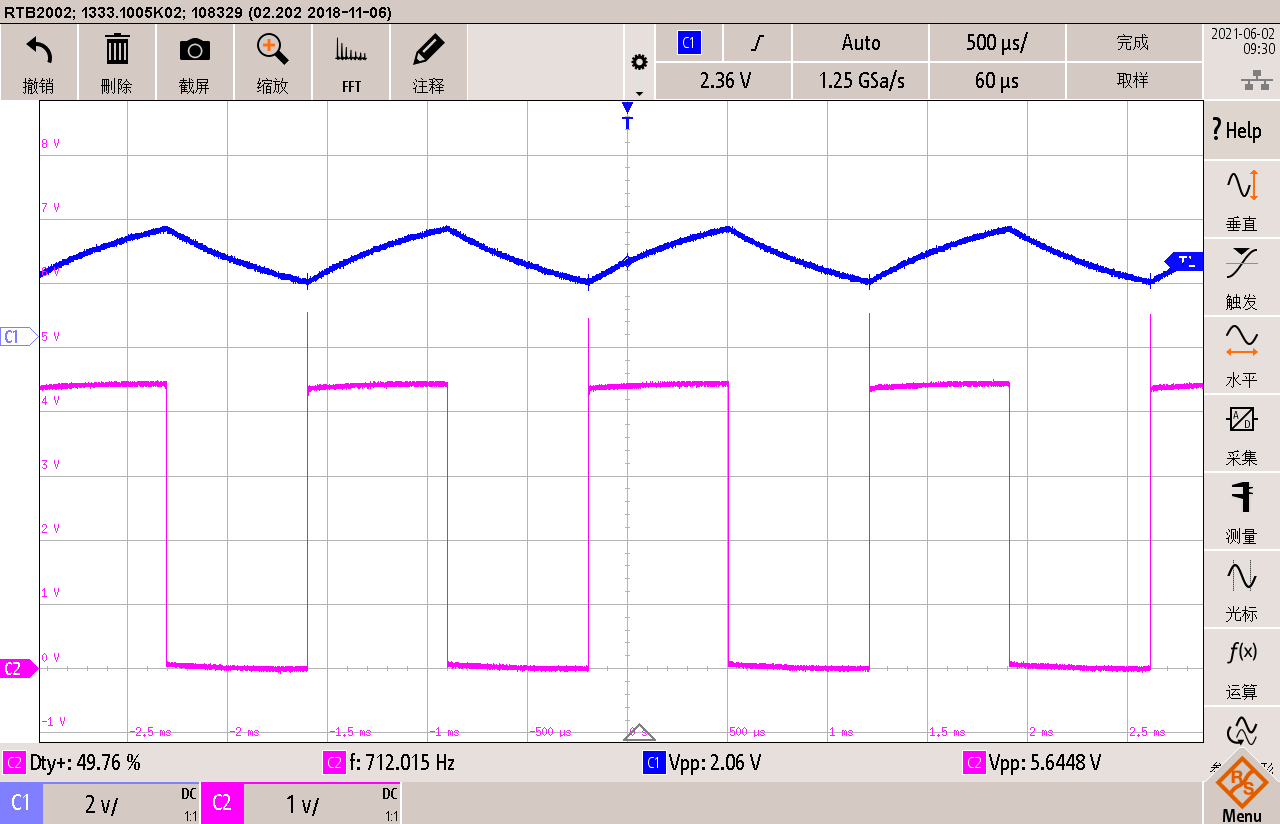
\includegraphics[width=3.5in]{H:/电子技术试验/4-23/SCR36.png}   
        \caption{占空比50\%}   
        \label{fig:side:a}   
    \end{figure}
\newpage
    调节$R_W$
    \begin{figure}[h]
        \begin{minipage}[t]{0.5\linewidth} % 如果一行放2个图,用0.5,如果3个图,用0.33  
          \centering   
          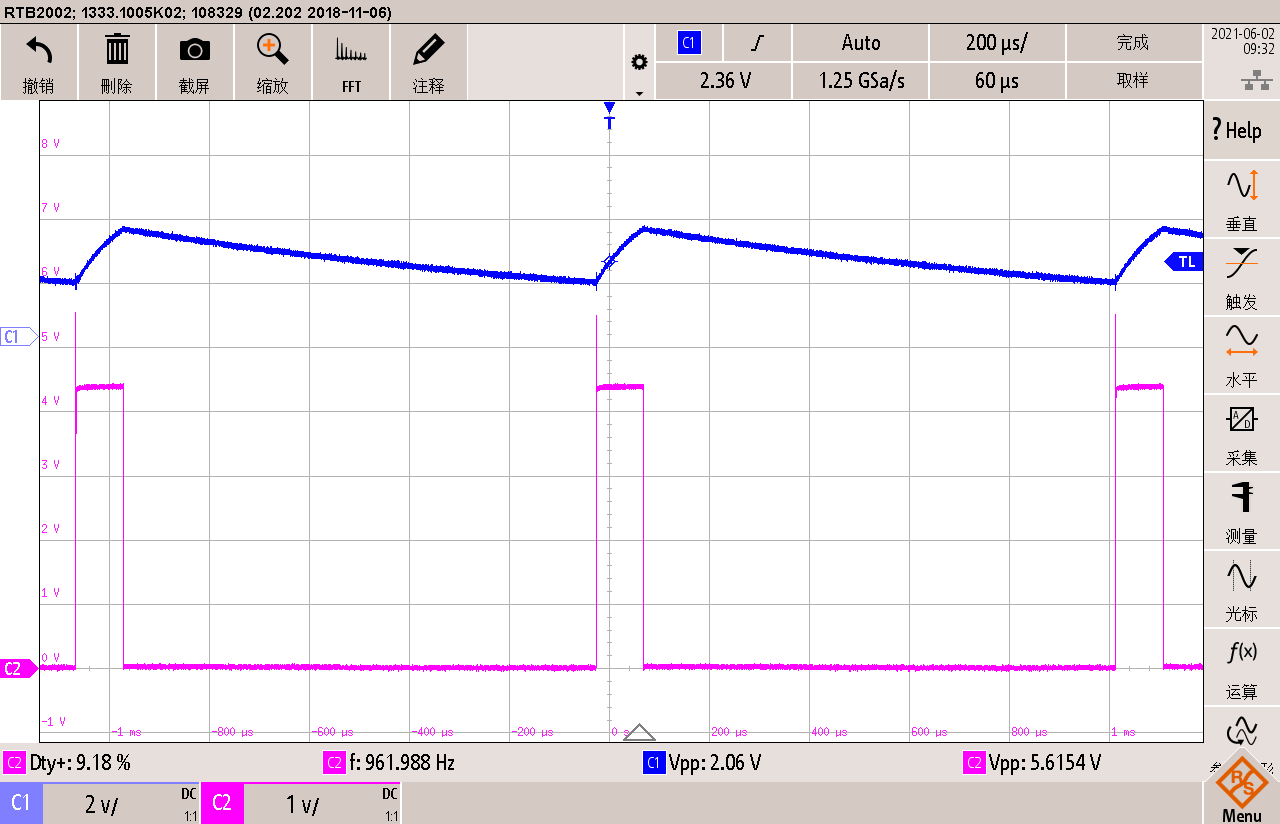
\includegraphics[width=3.5in]{H:/电子技术试验/4-23/SCR38.png}   
          \caption{$R_w=116.2k\Omega$}   
          \label{fig:side:a}   
        \end{minipage}%   
        \begin{minipage}[t]{0.5\linewidth}   
          \centering   
          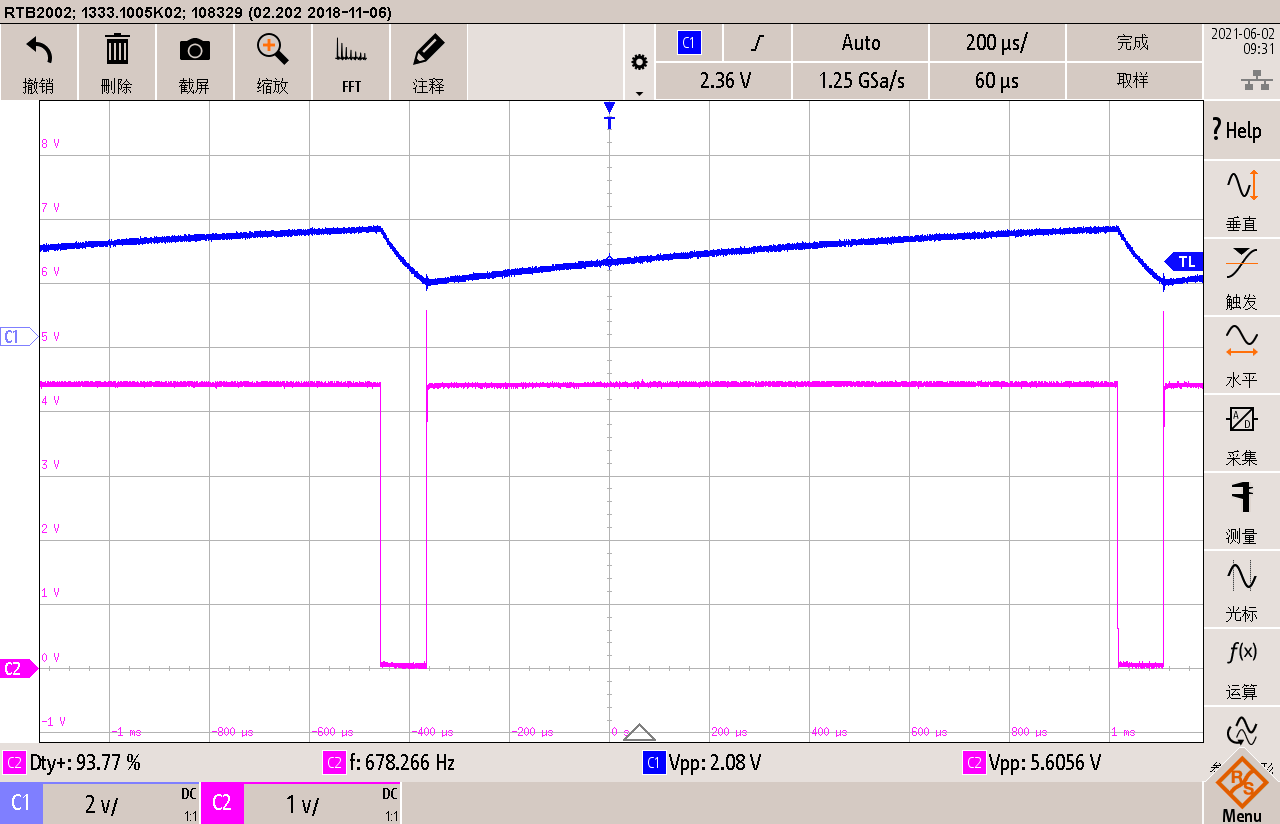
\includegraphics[width=3.5in]{H:/电子技术试验/4-23/SCR37.png}   
          \caption{$R_w=0k\Omega$}   
          \label{fig:side:b}   
        \end{minipage}   
      \end{figure}
 \section{\zihao{4} 误差处理}
(1)单稳态触发器\par 
\[ t_{w01}=1.1RC=13.90ms \]
\[ t_{w02}=1.1RC=1.1ms \]
\[ \Delta t_0=12.8ms \]
\[ \delta (t_{w1)}=\frac{ t_{w1}- t_{w01}}{t_{w1}}=15\%\]
\[ \delta (t_{w2})=\frac{ t_{w2}- t_{w02}}{t_{w2}}=45\%\]
\[ \delta (\Delta t)=\frac{ \Delta t- \Delta t_0}{\Delta t}=11\%\]
(2)多谐振荡器\par
\[q=\frac{t_{w1}}{T}=\frac{R_A+R_B}{R_A+2R_B}=55.4\%\]
\[\delta (q)=\frac{q-q_0}{q_0}=1\%\]

\par
单稳态触发器的$t_w$误差较大可能是芯片质量导致的。\par
多谐振荡器误差合理。\par
\section{结论}
(1)单稳电路的$t_w$由定时元件R与C参数决定,改变 R 与C 值,可以控制输出波形的宽度。\par
(2)多谐振荡器,通过改变电阻 $R_A$与 $R_B$和电容 C的参数,即可改变振荡信号频率。振荡信号的占空比由$R_A$与 $R_B$的参数决定,但无法小于 
50\%。\par
(3)在多谐振荡器电路上增加 1个电位器和2 个二极管可以实现调节占空比\par
\section{思考题}
(1)555定时器构成的单稳态触发器的脉冲宽度和周期由什么决定?R、C取值应怎样分配?为什么?\par
由外接RC的数值决定,C值不能过大,导致电路不稳定。
(2)若单稳态触发器的输入脉宽$t_i$大于$t_w$,时希望电路能正常工作,电路该怎样改进?\par 
可以先通过RC微分电路把输入脉宽变窄,然后再输入555定时器的2脚上。或改变$R_w$的最大阻值,或增大C的电容值,使$t_w$增大到大于$t_i$的程度。
(3)555定时器构成的多谐振荡器,其振荡周期和占空比的改变与哪些因素关?\par 
由于有
\[T=t_{w1}+t_{w2}=0.7(R_A+2R_B)C\]
\[q=\frac{t_{w1}}{T}=\frac{R_A+R_B}{R_A+2R_B}\]
因此周期和占空比与$R_A,R_B$的值有关\par 
(4)如何用 555 定时器构成施密特触发器?
将芯片的6脚和2脚相连,作为输入端Vi,由3脚或7脚挂接电阻RL及电源$V_{DD}$作为输出端,即能构成施密特触发器。
\begin{figure}[h]
  \centering   
  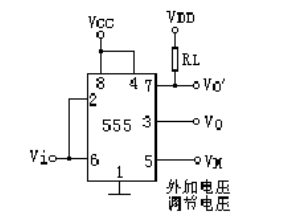
\includegraphics[width=3.5in]{H:/电子技术试验/4-23/7.png}   
  \caption{施密特触发器}   
  \label{fig:side:a}   
\end{figure}

\end{document}